\documentclass{article}
\usepackage{graphicx, tikz-cd, float, titlepic, booktabs} % Required for inserting images
\usepackage{amsmath, amssymb, amsthm, amsfonts, siunitx, physics, gensymb}
\AtBeginDocument{\RenewCommandCopy\qty\SI}
\usepackage[version=4]{mhchem}
\usepackage[most,many,breakable]{tcolorbox}
\usepackage{xcolor, fancyhdr, varwidth}
\usepackage[Glenn]{fncychap}
%Options: Sonny, Lenny, Glenn, Conny, Rejne, Bjarne, Bjornstrup
\usepackage{hyperref, cleveref}
\usepackage{icomma, enumitem} %comma as decimal and continue enumerate with [resume]
\usepackage[danish]{babel}
%%%%%%%%%%%%%%%%%%%%%%%%%%%%%%
% SELF MADE COLORS
%%%%%%%%%%%%%%%%%%%%%%%%%%%%%%
\definecolor{myg}{RGB}{56, 140, 70}
\definecolor{myb}{RGB}{45, 111, 177}
\definecolor{myr}{RGB}{199, 68, 64}
\definecolor{mytheorembg}{HTML}{F2F2F9}
\definecolor{mytheoremfr}{HTML}{00007B}
\definecolor{mylenmabg}{HTML}{FFFAF8}
\definecolor{mylenmafr}{HTML}{983b0f}
\definecolor{mypropbg}{HTML}{f2fbfc}
\definecolor{mypropfr}{HTML}{191971}
\definecolor{myexamplebg}{HTML}{F2FBF8}
\definecolor{myexamplefr}{HTML}{88D6D1}
\definecolor{myexampleti}{HTML}{2A7F7F}
\definecolor{mydefinitbg}{HTML}{E5E5FF}
\definecolor{mydefinitfr}{HTML}{3F3FA3}
\definecolor{notesgreen}{RGB}{0,162,0}
\definecolor{myp}{RGB}{197, 92, 212}
\definecolor{mygr}{HTML}{2C3338}
\definecolor{myred}{RGB}{127,0,0}
\definecolor{myyellow}{RGB}{169,121,69}
\definecolor{myexercisebg}{HTML}{F2FBF8}
\definecolor{myexercisefg}{HTML}{88D6D1}
%%%%%%%%%%%%%%%%%%%%%%%%%%%%%%%%%%%%%%%%%%%%%%%%%%%%%%%%%%%%%%%%%%%%%%
% Box environments for theorems and problems
%%%%%%%%%%%%%%%%%%%%%%%%%%%%%%%%%%%%%%%%%%%%%%%%%%%%%%%%%%%%%%%%%%%%%
\setlength{\parindent}{1cm}
%================================
% Question BOX
%================================
\makeatletter
\newtcbtheorem{question}{Opgave}{enhanced,
	breakable,
	colback=white,
	colframe=myb!80!black,
	attach boxed title to top left={yshift*=-\tcboxedtitleheight},
	fonttitle=\bfseries,
	title={#2},
	boxed title size=title,
	boxed title style={%
			sharp corners,
			rounded corners=northwest,
			colback=tcbcolframe,
			boxrule=0pt,
		},
	underlay boxed title={%
			\path[fill=tcbcolframe] (title.south west)--(title.south east)
			to[out=0, in=180] ([xshift=5mm]title.east)--
			(title.center-|frame.east)
			[rounded corners=\kvtcb@arc] |-
			(frame.north) -| cycle;
		},
	#1
}{def}
\makeatother
%================================
% DEFINITION BOX
%================================

\newtcbtheorem[]{Definition}{Definition}{enhanced,
	before skip=2mm,after skip=2mm, colback=red!5,colframe=red!80!black,boxrule=0.5mm,
	attach boxed title to top left={xshift=1cm,yshift*=1mm-\tcboxedtitleheight}, varwidth boxed title*=-3cm,
	boxed title style={frame code={
					\path[fill=tcbcolback]
					([yshift=-1mm,xshift=-1mm]frame.north west)
					arc[start angle=0,end angle=180,radius=1mm]
					([yshift=-1mm,xshift=1mm]frame.north east)
					arc[start angle=180,end angle=0,radius=1mm];
					\path[left color=tcbcolback!60!black,right color=tcbcolback!60!black,
						middle color=tcbcolback!80!black]
					([xshift=-2mm]frame.north west) -- ([xshift=2mm]frame.north east)
					[rounded corners=1mm]-- ([xshift=1mm,yshift=-1mm]frame.north east)
					-- (frame.south east) -- (frame.south west)
					-- ([xshift=-1mm,yshift=-1mm]frame.north west)
					[sharp corners]-- cycle;
				},interior engine=empty,
		},
	fonttitle=\bfseries,
	title={#2},#1}{def}
\newtcbtheorem[]{definition}{Definition}{enhanced,
	before skip=2mm,after skip=2mm, colback=red!5,colframe=red!80!black,boxrule=0.5mm,
	attach boxed title to top left={xshift=1cm,yshift*=1mm-\tcboxedtitleheight}, varwidth boxed title*=-3cm,
	boxed title style={frame code={
					\path[fill=tcbcolback]
					([yshift=-1mm,xshift=-1mm]frame.north west)
					arc[start angle=0,end angle=180,radius=1mm]
					([yshift=-1mm,xshift=1mm]frame.north east)
					arc[start angle=180,end angle=0,radius=1mm];
					\path[left color=tcbcolback!60!black,right color=tcbcolback!60!black,
						middle color=tcbcolback!80!black]
					([xshift=-2mm]frame.north west) -- ([xshift=2mm]frame.north east)
					[rounded corners=1mm]-- ([xshift=1mm,yshift=-1mm]frame.north east)
					-- (frame.south east) -- (frame.south west)
					-- ([xshift=-1mm,yshift=-1mm]frame.north west)
					[sharp corners]-- cycle;
				},interior engine=empty,
		},
	fonttitle=\bfseries,
	title={#2},#1}{def}

\newtcbtheorem{theo}%
    {Theorem}{}{theorem}
\newtcolorbox{prob}[1]{colback=red!5!white,colframe=red!50!black,fonttitle=\bfseries,title={#1}}
%================================
% NOTE BOX
%================================

\usetikzlibrary{arrows,calc,shadows.blur}
\tcbuselibrary{skins}
\newtcolorbox{note}[1][]{%
	enhanced jigsaw,
	colback=gray!20!white,%
	colframe=gray!80!black,
	size=small,
	boxrule=1pt,
	title=\textbf{Note:},
	halign title=flush center,
	coltitle=black,
	breakable,
	drop shadow=black!50!white,
	attach boxed title to top left={xshift=1cm,yshift=-\tcboxedtitleheight/2,yshifttext=-\tcboxedtitleheight/2},
	minipage boxed title=1.5cm,
	boxed title style={%
			colback=white,
			size=fbox,
			boxrule=1pt,
			boxsep=2pt,
			underlay={%
					\coordinate (dotA) at ($(interior.west) + (-0.5pt,0)$);
					\coordinate (dotB) at ($(interior.east) + (0.5pt,0)$);
					\begin{scope}
						\clip (interior.north west) rectangle ([xshift=3ex]interior.east);
						\filldraw [white, blur shadow={shadow opacity=60, shadow yshift=-.75ex}, rounded corners=2pt] (interior.north west) rectangle (interior.south east);
					\end{scope}
					\begin{scope}[gray!80!black]
						\fill (dotA) circle (2pt);
						\fill (dotB) circle (2pt);
					\end{scope}
				},
		},
	#1,
}

%%%%%%%%%%%%%%%%%%%%%%%%%%%%%%%%%%%%%%%%%%%%%%%%%%%%%%%%%%%%%%%%%
% SELF MADE COMMANDS
%%%%%%%%%%%%%%%%%%%%%%%%%%%%%%
\newcommand{\sol}{\setlength{\parindent}{0cm}\textbf{\textit{Løsning:}}\setlength{\parindent}{1cm}}
%%%%%%%%%%%%%%%%%%%%%%%%%%%%%%%%%
\usepackage[tmargin=2cm,rmargin=1in,lmargin=1in,margin=0.85in,bmargin=2cm,footskip=.2in]{geometry}\pagestyle{fancy}
\lhead{Minrui Kevin Zhou 2.b}
\rhead{Matematikaflevering 23}

\title{Aflevering 23\\
{\Large \textbf{2.b mat A}}}
\author{Kevin Zhou}
\date{Januar 2023}

\begin{document}
\maketitle
\section*{Bedømmelseskriterier:}
\begin{itemize}
    \setlength\itemsep{3cm}
    \Large
    \item  Redegørelse og dokumentation for metode
    \item Figurer, grafer og andre illustrationer
    \item Notation og layout
    \item Formidling og forklaring
\end{itemize}
\pagebreak
\begin{question}{}{}
  Med et spirometer har man målt, hvordan luftmængden i lungerne hos en bestemt person afhænger af tiden. I en model kan luftmængden beskrives ved
$$
f(t)=3,2+0,4 \cdot \sin (1,25 \cdot t), \quad 0 \leq t \leq 5
$$
hvor $f(t)$ betegner luftmængden i lungerne (målt i liter) til tidspunktet $t$ (målt i sekunder fra begyndelsen af vejrtrækningen).
\begin{itemize}
  \item[a.] Tegn grafen for $f$.
  \item[b.] Bestem den maksimale luftmængde i lungerne ifølge modellen.
  \item[c.] Bestem perioden $T$.
  \item[d.] Benyt modellen til at bestemme de tidspunkter, hvor luftmængden er 3,5 liter.
  \item[e.] Bestem $f^{\prime}(2)$, og giv en fortolkning af dette tal.
\end{itemize}
\end{question}
\sol \\ 
\textbf{a.} 
Grafen for $f$ kan ses i \cref{fig:lunger}. 
\begin{figure}[H]
\begin{center}
  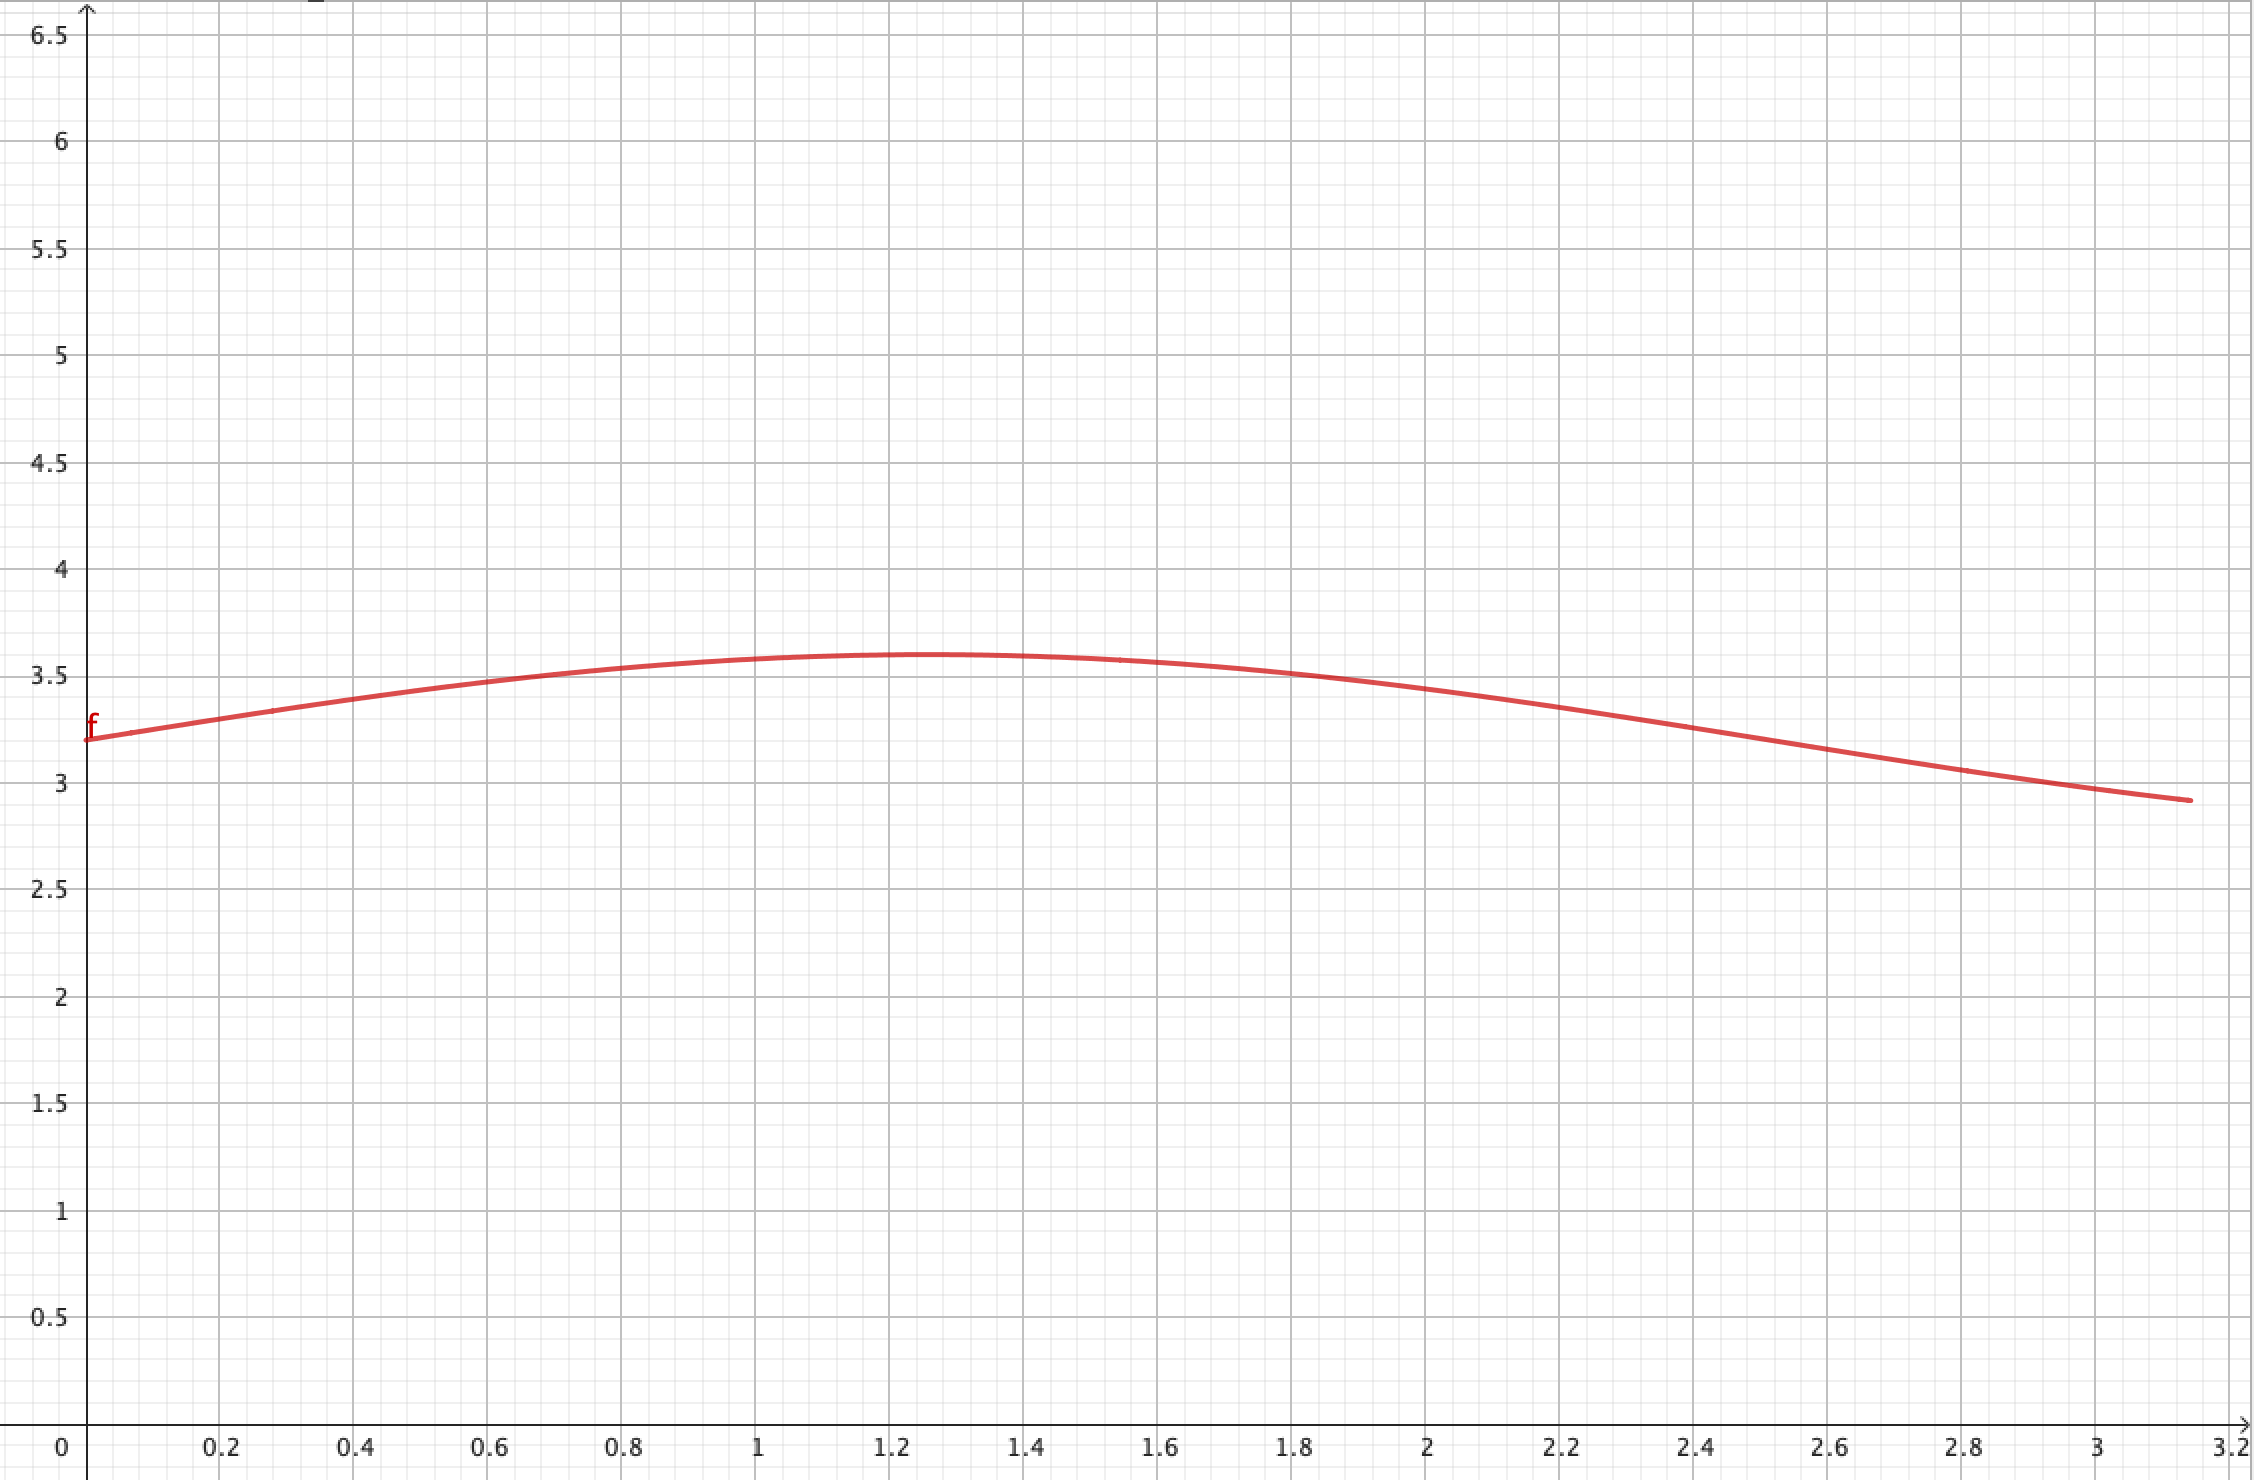
\includegraphics[width=\textwidth]{lunge.png}
\end{center}
\caption{Grafen for $f$ tegnet i GeoGebra }
\label{fig:lunger}
\end{figure}
\noindent \textbf{b.} 
Når luftmængden i lungerne er maksimal ifølge modellen, så må der gælde, at $0,4\cdot \sin \left(1,25\cdot t\right) $ er så stor som mulig. 
Dette er blandt andet tilfældet, når 
\[
1,25 \cdot t=\frac{1}{2}\pi \iff t=\frac{\pi}{1,25\cdot 2} \in [0;5]
\] 
Vi har at $Vm(\sin)=[-1;1]$
Altså må den maksimale luftmængde i lungerne være
\[
3,2+0,4\cdot \sin \left(\frac{1}{2}\pi\right) =3,2+0,4=3,6
\] 
Ifølge modellen er den maksimale luftmængde i lungerne altså $3,6 \;\unit{L} $.\\[1ex]
\textbf{c.} Fra (128) fra formelsamlingen får vi, at perioden for funktionen $f$ er
\[
T=\frac{2\pi}{1,25}\approx5,03
\] 
\textbf{d.} De tidspunkter, $t$, hvor luftmængden er 3,5 liter må have $f(t)=3,5$.
\begin{equation*}
\begin{split}
  3,2+0,4\cdot \sin \left(1,25\cdot t\right) =3,5 \land 0\leq t \leq 5 &\iff \sin \left(1,25 t\right) =\frac{3}{4} \land 0\leq t \leq 5\\ 
  &\implies t=\frac{\sin^{-1}\left(\frac{3}{4}\right) }{1,25} \approx 0,68\lor t=\frac{\pi-\sin^{-1}\left(\frac{3}{4}\right)}{1,25} \approx 1,83
\end{split}
\end{equation*}
Altså må de tidspunkter, hvor luftmængden er 3,5 liter være efter 0,68 sekunder og efter 1,83 sekunder.\\[1ex]
\textbf{e.} 
Vi finder den afledede funktion for $f$ mht. $t$ med kædereglen. 
\begin{equation*}
\begin{split}
  f'(t)&=0,4\cdot \cos \left(1,25\cdot t\right) \cdot 1,25 \\ 
  &= 0,5 \cdot \cos \left(1,25\cdot t\right)
\end{split}
\end{equation*}
Vi tager nu den afledede funktion for $f$ af 2. 
\begin{equation*}
\begin{split}
  f'(2)&=0,5 \cdot \cos \left(1,25\cdot 2\right) \\
  &\approx -0,40
\end{split}
\end{equation*}
Dette tal fortæller, at luftmængden i personens lunger efter to sekunder aftager med 0,40 liter per sekund.
\begin{question}{}{}
  En funktion $f:[0;2\pi]\to \mathbb{R}$ er bestemt ved
  \[
  f(x)= x+2\sin x
  \] 
  \begin{itemize}
    \item[a.] Løs ligningen $f'(x)=0$ og gør rede for monotoniforholdene for $f$. 
  \end{itemize}
\end{question}
\sol \\ 
\textbf{a.}
Vi finder den afledede funktion for $f$.
\[
f'(x)=1+2\cdot \cos x
\] 
Når $f'(x)=0$, så gælder der, at
\begin{equation*}
\begin{split}
  1+2\cdot \cos x=0 \land 0\leq x \leq 2\pi &\iff \cos(x)=-\frac{1}{2}\land 0\leq x \leq 2\pi \\ 
  &\implies x=\cos^{-1}\left(-\frac{1}{2}\right) \lor x=2\pi - \cos^{-1}\left(-\frac{1}{2}\right) \\ 
  &\iff x=\frac{2\pi}{3}\lor x=\frac{4\pi}{3}
\end{split}
\end{equation*}
Vi finder da den dobbeltafledede funktion for $f$.
\[
f''(x)=\dv{x} \left(f'(x)\right) =-2\sin x
\] 
Vi tager den dobbeltafledede funktion for $f$ af løsningerne til $f'(x)=0$ for at se, om disse er maksimumssteder, minimumssteder eller andet. 
\begin{equation*}
\begin{split}
  f''\left(\frac{2\pi}{3}\right)&=-\sqrt{3} <0 \\ 
  f''\left(\frac{4\pi}{3}\right)&=\sqrt{3} <0
\end{split}
\end{equation*}
Altså er $\frac{2\pi}{3}$ et maksimumssted, hvor $\frac{4\pi}{3}$ er et minimumssted. 
Vi får altså følgende om monotoniforholdene for $f$.
\begin{equation*}
\begin{split}
  &f \text{ er voksende på intervallet } \left[0;\frac{2\pi}{3}\right]\\ 
  &f \text{ er aftagende på intervallet } \left[\frac{2\pi}{3};\frac{4\pi}{3}\right] \\ 
  &f \text{ er voksende på intervallet } \left[\frac{4\pi}{3};2\pi\right]
\end{split}
\end{equation*}
\begin{question}{}{}
  I et koordinatsystem er tre punkter givet ved $A(x,0),\;B(x,4-x)$ og $C(0,2-x)$, hvor $0<x<4$.
  \begin{itemize}
    \item[a.] Bestem arealet af trekant ABC, når $x=3$.
    \item[b.] Bestem $x$, så arealet af trekant ABC er størst muligt. 
  \end{itemize}
\end{question}
\sol \\ 
\textbf{a.} 
Vi har
\begin{equation*}
\begin{split}
  \overrightarrow{\textbf{AC}} &=\begin{pmatrix} -3\\ -1 \end{pmatrix}\\ 
    \overrightarrow{\textbf{AB}} &= \begin{pmatrix} 0 \\1  \end{pmatrix} 
\end{split}
\end{equation*}
Arealet af trekanten når $x=3$ må være 
\begin{equation*}
\begin{split}
  A&=\frac{1}{2}\left| \det \left(\overrightarrow{\textbf{AB}} ,\;\overrightarrow{\textbf{AC}} \right)  \right| \\ 
  &=\frac{1}{2}\cdot \left| \left(0-3\right)  \right| \\ 
  &=\frac{3}{2}
\end{split}
\end{equation*}
Altså må arealet af trekanten være $\frac{3}{2}$.\\[1ex]
\textbf{b.} 
Arealet af trekant ABC kan beskrives ved
\begin{equation*}
\begin{split}
  A&=\frac{1}{2}\left| (b_1-a_1)\cdot (c_2-a_2)-(b_2-a_2)\cdot (c_1-a_1) \right| \\ 
  &=\frac{1}{2}\left| (x-x)\cdot (2-2x)-(4-x)\cdot (-x) \right| \\ 
  &=\left| 2x-\frac{1}{2}x^2 \right| 
\end{split}
\end{equation*}
hvor $A=(a_1,a_2),\;B=(b_1,b_2)$ og $C=(c_1,c_2)$.
Vi differentierer dette udtryk med kædereglen.
\begin{equation*}
\begin{split}
  \dv{A}{x} &= \frac{2x-\frac{x^2}{2}}{\left| 2x-\frac{x^2}{2} \right| }\cdot \left(2-x\right) \\ 
  &=\frac{\left(4x-x^2\right) \cdot \left(2-x\right) }{\left| 4x-x^2 \right| }
\end{split}
\end{equation*}
Vi antager, at $\left| 4x-x^2 \right| \neq 0$, og løser ligningen $\dv{A}{x}=0 $ med nulreglen. 
\begin{equation*}
\begin{split}
  \frac{\left(4x-x^2\right) \cdot \left(2-x\right) }{\left| 4x-x^2 \right| }=0 &\implies x\cdot (4-x) \cdot (2-x)=0 \\ 
  &\implies x=2
\end{split}
\end{equation*}
Læg mærke til, at 4 og 0 ikke er gyldige løsninger, grundet modstrid med vores antagelse. 
Disse tilhører heller ikke $]0;4[$.

Lad $A:]0;4[ \to \mathbb{R} $ være funktionen givet ved 
\[
A(x)=\left| 2x-\frac{1}{2}x^2 \right| 
\] 
Så er $A$ differentiabel i $x \in ]0;4[$.
Altså er $A$ kontinuert. 
Derfor må $A'(x)$ have konstant fortegn i intervallerne $]0;2[$ og $]2;4[$.
Vi finder da fortegnet ved at vælge tilfældige $x$-værdier i de to intervaller og udregne $A'(x)$.
\begin{equation*}
\begin{split}
  A'(1)&=1>0 \\ 
  A'(3)&=-1<0
\end{split}
\end{equation*}
Altså må 2 være et maksimumssted.
Arealet af trekant $ABC$ er da størst muligt, når $x=2$.
\end{document}
